\documentclass[11pt,a4paper]{article}
\usepackage[T1]{fontenc}
\usepackage[utf8]{inputenc}
\usepackage{lmodern}
\usepackage{textcomp}
\usepackage[left=1.8cm,right=1.8cm,top=3.0cm,bottom=2.2cm,headheight=36pt,headsep=12pt]{geometry}
\usepackage{multicol}
\usepackage{xcolor}
\usepackage{fancyhdr}\usepackage{tikz}
\usepackage{graphicx}
\usepackage{array}
\usepackage{amsmath,amssymb}
\usepackage{setspace}
\usepackage{longtable}
\graphicspath{{../}}
\definecolor{ygreen}{RGB}{46,139,87}\definecolor{dgreen}{RGB}{28,90,56}
\renewcommand{\normalsize}{\fontsize{10.9}{13.4}\selectfont}
\renewcommand{\familydefault}{\rmdefault}
\setlength{\parindent}{0pt}
\setlength{\columnsep}{0.8cm}
\setlength{\columnseprule}{0.4pt}
\setlength{\multicolsep}{3pt plus 1pt minus 1pt}
\renewcommand{\textsubscript}[1]{\ensuremath{_{\text{\fontsize{8}{8}\selectfont #1}}}}
\renewcommand{\textsuperscript}[1]{\ensuremath{^{\text{\fontsize{8}{8}\selectfont #1}}}}
\newcommand{\qn}[1]{\textbf{\fontsize{11.5}{13}\selectfont #1}}
\newcommand{\qsep}{\par\vspace{13pt}}
\newcommand{\fwrule}{\par\vspace{5pt}\noindent\rule{\linewidth}{1.4pt}\par\vspace{7pt}}
\newsavebox{\fitb}
\newcommand{\fitbox}[1]{\sbox{\fitb}{#1}\ifdim\wd\fitb>\linewidth\resizebox{\linewidth}{!}{\usebox{\fitb}}\else\usebox{\fitb}\fi}
\newcommand{\diqqat}[1]{\par\smallskip\noindent\textbf{Diqqat!} #1\par\medskip}
\newcommand{\javob}{\par\nopagebreak[4]\smallskip\noindent\textbf{Javob:} \rule[-2pt]{7.5cm}{0.4pt}\par\smallskip\noindent\textbf{Diqqat!} Javobingizni javoblar varaqasiga ko`chirib yozing.\par\medskip}
\pagestyle{fancy}
\fancyhf{}
\renewcommand{\headrulewidth}{1.6pt}\renewcommand{\headrule}{{\color{ygreen}\hrule height 1.6pt width\headwidth}}
\newcommand{\hdrlogo}{
\begin{tikzpicture}[baseline=0pt]\fill[ygreen,rounded corners=3pt] (0,0) rectangle (0.95,0.95);\node[white,font=\fontsize{24}{26}\bfseries\selectfont] at (0.475,0.47){K};\node[anchor=west,font=\fontsize{16}{18}\bfseries\selectfont,text=dgreen] at (1.15,0.66){KIMYO};\node[anchor=west,font=\footnotesize\scshape,text=gray] at (1.15,0.2){Milliy sertifikat\ \ 2026};\end{tikzpicture}}
\newcommand{\hdrpill}[1]{\begin{tikzpicture}[baseline=0pt]\node[fill=ygreen,text=white,rounded corners=8pt,inner xsep=10pt,inner ysep=5pt,font=\fontsize{13}{15}\bfseries\selectfont] at (0,0.475){#1};\end{tikzpicture}}
\fancyhead[L]{\hdrlogo}
\fancyhead[R]{\hdrpill{5-variant}}

\fancyfoot[C]{\thepage}
\fancypagestyle{first}{\fancyhf{}\renewcommand{\headrulewidth}{1.6pt}\renewcommand{\headrule}{{\color{ygreen}\hrule height 1.6pt width\headwidth}}\fancyhead[L]{\hdrlogo}\fancyhead[R]{\hdrpill{5-variant}}\fancyfoot[C]{\thepage}}
\begin{document}
\normalsize
\thispagestyle{first}
\noindent\textit{Davriy jadvaldan foydalanish mumkin.}
\par\smallskip
\begin{multicols}{2}
\noindent\qn{1.} Quyidagi tuzlarning qaysilari suvli eritmasi kislotali muhitga ega? 1) CH\textsubscript{3}COONa; 2) Na\textsubscript{2}SO\textsubscript{4}; 3) FeCl\textsubscript{3}; 4) Na\textsubscript{2}CO\textsubscript{3}

\noindent A)~\textsl{2} \hfill B)~\textsl{3} \hfill C)~\textsl{2, 4} \hfill D)~\textsl{1, 3}\par
\qsep
\noindent\qn{2.} 2NO + O\textsubscript{2} $\rightleftarrows$ 2NO\textsubscript{2} reaksiyasi 2 l hajmli idishda o`tkazildi. Ma'lumotlar jadvalda berilgan:
\begin{center}
\renewcommand{\arraystretch}{1.15}
\fitbox{\begin{tabular}{|c|c|c|c|}\hline
\textbf{Modda} & \textbf{NO} & \textbf{O\textsubscript{2}} & \textbf{NO\textsubscript{2}} \\ \hline
Boshlang`ich, mol & 4 & 6 & 0 \\ \hline
Muvozanatda, mol & --- & --- & 3 \\ \hline
\end{tabular}}
\end{center}
NO ning necha foizi reaksiyaga \textbf{kirishganini aniqlang.}

\noindent A)~\textsl{37,5} \hfill B)~\textsl{112,5} \hfill C)~\textsl{25} \hfill D)~\textsl{75}\par
\qsep
\noindent\qn{3.} N\textsubscript{2}O\textsubscript{4} $\rightleftarrows$ 2NO\textsubscript{2} reaksiyasi 1 l hajmli idishda o`tkazildi. Ma'lumotlar jadvalda berilgan:
\begin{center}
\renewcommand{\arraystretch}{1.15}
\fitbox{\begin{tabular}{|c|c|c|}\hline
\textbf{Modda} & \textbf{N\textsubscript{2}O\textsubscript{4}} & \textbf{NO\textsubscript{2}} \\ \hline
Boshlang`ich, mol & 4 & 0 \\ \hline
Muvozanatda, mol & --- & 1 \\ \hline
\end{tabular}}
\end{center}
Muvozanat \textbf{konstantasini (K) hisoblang.}

\noindent A)~\textsl{0,571} \hfill B)~\textsl{0,143} \hfill C)~\textsl{0,286} \hfill D)~\textsl{3,5}\par
\qsep
\noindent\qn{4.} CH\textsubscript{3}--CH\textsubscript{2}--CH\textsubscript{3} molekulasidagi $\sigma$ va $\pi$ bog`lar \textbf{sonini aniqlang.}

\noindent A)~\textsl{9 va 0} \hfill B)~\textsl{10 va 1} \hfill C)~\textsl{10 va 0} \hfill D)~\textsl{11 va 0}\par
\qsep
\noindent\qn{5.} 1 mol CH\textsubscript{4} tarkibidagi atomlar \textbf{sonini toping} (N\textsubscript{A} = 6,02$\cdot$10\textsuperscript{23}). Javobni 10\textsuperscript{23} birligida yozing.

\noindent A)~\textsl{6,02} \hfill B)~\textsl{1,505} \hfill C)~\textsl{0,602} \hfill D)~\textsl{3,01}\par
\qsep
\noindent\qn{6.} Zn + HNO\textsubscript{3} $\to$ Zn(NO\textsubscript{3})\textsubscript{2} + NH\textsubscript{4}NO\textsubscript{3} + H\textsubscript{2}O reaksiya tenglamasini tenglang va barcha koeffitsiyentlar \textbf{yig`indisini aniqlang.}

\noindent A)~\textsl{23} \hfill B)~\textsl{21} \hfill C)~\textsl{24} \hfill D)~\textsl{22}\par
\qsep
\noindent\qn{7.} Na\textsubscript{2}SO\textsubscript{4} ning suvli eritmasi inert elektrodlar bilan elektroliz qilinganda qaysi moddalar ajraladi?

\noindent\begin{tabular}{@{}p{0.47\linewidth}@{}p{0.47\linewidth}@{}}
A)~\textsl{Zn, H\textsubscript{2} va O\textsubscript{2}} & B)~\textsl{H\textsubscript{2} va O\textsubscript{2}} \\
C)~\textsl{H\textsubscript{2}, Cl\textsubscript{2} va NaOH} & D)~\textsl{Ag va O\textsubscript{2}} \\
\end{tabular}\par
\qsep
\noindent\qn{8.} Reaksiyaning energetik diagrammasi berilgan (boshlang`ich moddalar energiyasi 20, mahsulotlar 90 kJ/mol).
\begin{center}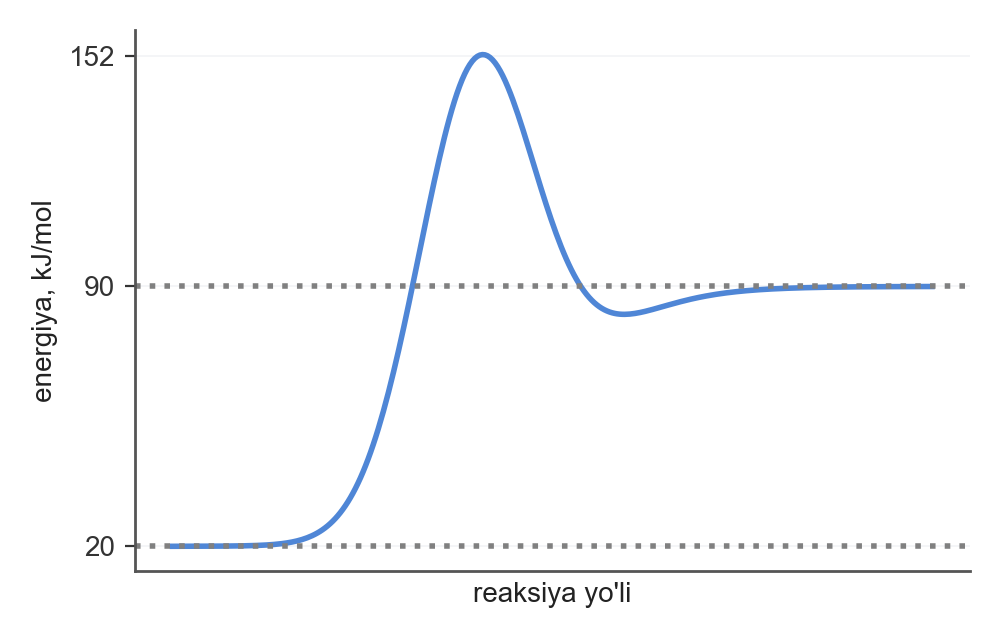
\includegraphics[width=0.86\linewidth]{rasmlar/gen/en_v05_0.png}\end{center}
To`g`ri reaksiyaning aktivlanish \textbf{energiyasini (kJ/mol) aniqlang.}

\noindent A)~\textsl{202} \hfill B)~\textsl{70} \hfill C)~\textsl{132} \hfill D)~\textsl{264}\par
\qsep
\noindent\qn{9.} Mn\textsubscript{2}O\textsubscript{7} tarkibida marganes ning \textbf{valentligini aniqlang.}

\noindent A)~\textsl{VII} \hfill B)~\textsl{II} \hfill C)~\textsl{\textit{V}} \hfill D)~\textsl{III}\par
\qsep
\noindent\qn{10.} Mis atomida d-pog`onachadagi elektronlar \textbf{sonini aniqlang} (\textit{Z} = 29).

\noindent A)~\textsl{11} \hfill B)~\textsl{9} \hfill C)~\textsl{12} \hfill D)~\textsl{10}\par
\qsep
\noindent\qn{11.} Cu + H\textsubscript{2}SO\textsubscript{4} $\to$ CuSO\textsubscript{4} + SO\textsubscript{2} + H\textsubscript{2}O reaksiyasida 2 mol Cu erisa, H\textsubscript{2}SO\textsubscript{4} ning necha moli oksidlovchi vazifasini bajaradi?

\noindent A)~\textsl{4} \hfill B)~\textsl{2} \hfill C)~\textsl{1} \hfill D)~\textsl{3}\par
\qsep
\noindent\qn{12.} HC$\equiv$C--CH=CH\textsubscript{2} molekulasida sp gibridlangan uglerod atomlari nechta?

\noindent A)~\textsl{3} \hfill B)~\textsl{4} \hfill C)~\textsl{1} \hfill D)~\textsl{2}\par
\qsep
\noindent\qn{13.} H\textsubscript{2} + I\textsubscript{2} $\rightleftarrows$ 2HI reaksiyada muvozanat holatida [H\textsubscript{2}] = 2, [I\textsubscript{2}] = 0,5, [HI] = 2 mol/l. Muvozanat \textbf{konstantasini (K) hisoblang.}

\noindent A)~\textsl{8} \hfill B)~\textsl{2} \hfill C)~\textsl{1,6} \hfill D)~\textsl{4}\par
\qsep
\noindent\qn{14.} Nodir gazlar haqida qaysi fikrlar to`g`ri? 1) Nodir gazlar kimyoviy jihatdan juda faol; 2) Geliy eng yengil inert gaz; 3) Argon havoning hajmi bo`yicha eng ko`p uchraydigan inert gazi; 4) Geliyda 8 ta tashqi elektron bor

\noindent A)~\textsl{3} \hfill B)~\textsl{2, 3} \hfill C)~\textsl{4} \hfill D)~\textsl{2, 3, 4}\par
\qsep
\noindent\qn{15.} 10,1 g KNO\textsubscript{3} to`liq parchalanguncha qizdirildi. Qattiq qoldiq \textbf{massasini (g) aniqlang.}

\noindent A)~\textsl{8,5} \hfill B)~\textsl{10,1} \hfill C)~\textsl{17} \hfill D)~\textsl{4,25}\par
\qsep
\noindent\qn{16.} Qaysi juftliklar o`zaro reaksiyaga kirishadi? 1) Ag va H\textsubscript{2}SO\textsubscript{4}(suyult.); 2) CO\textsubscript{2} va CaO; 3) Na\textsubscript{2}CO\textsubscript{3} va HCl; 4) Fe va HCl

\noindent A)~\textsl{3, 4} \hfill B)~\textsl{2, 3, 4} \hfill C)~\textsl{1, 3, 4} \hfill D)~\textsl{1, 3}\par
\qsep
\noindent\qn{17.} 44,8 l (n.sh.) ammiakdan nitrat kislota olindi (jami unum 80\%). Kislota \textbf{massasini (g) aniqlang.}

\noindent A)~\textsl{126} \hfill B)~\textsl{201,6} \hfill C)~\textsl{50,4} \hfill D)~\textsl{100,8}\par
\qsep
\noindent\qn{18.} 0,3 mol NaOH tutgan eritmadan 0,15 mol CO\textsubscript{2} o`tkazildi. Hosil bo`lgan Na\textsubscript{2}CO\textsubscript{3} \textbf{massasini (g) aniqlang.}

\noindent A)~\textsl{31,8} \hfill B)~\textsl{15,9} \hfill C)~\textsl{7,95} \hfill D)~\textsl{12}\par
\qsep
\noindent\qn{19.} 11,7 g NaCl ga mo`l kons. H\textsubscript{2}SO\textsubscript{4} ta'sir ettirilib, ajralgan HCl 500 g suvda eritildi. Hosil bo`lgan xlorid kislota massa \textbf{ulushini (\%) aniqlang.}

\noindent A)~\textsl{1,46} \hfill B)~\textsl{2,88} \hfill C)~\textsl{1,44} \hfill D)~\textsl{0,72}\par
\qsep
\noindent\qn{20.} Rasmda aromatik uglevodorod hosilasining tuzilish formulasi berilgan.
\begin{center}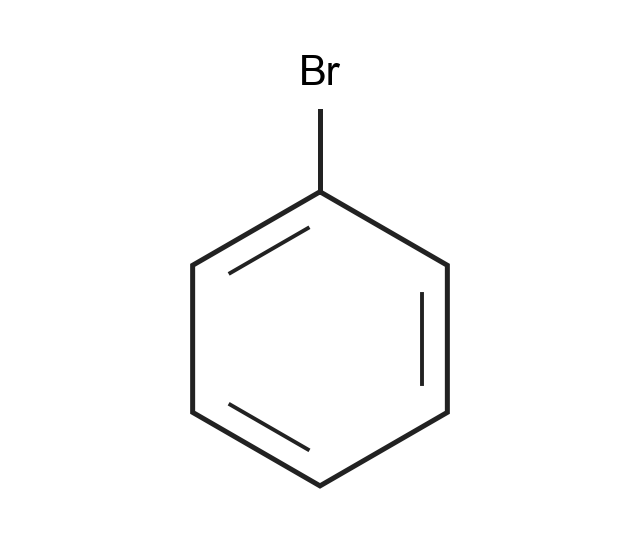
\includegraphics[width=0.86\linewidth]{rasmlar/gen/bz_539431.png}\end{center}
Birikmaning \textbf{nomini toping.}

\noindent\begin{tabular}{@{}p{0.47\linewidth}@{}p{0.47\linewidth}@{}}
A)~\textsl{toluol} & B)~\textsl{fenol} \\
C)~\textsl{brombenzol} & D)~\textsl{benzoy kislota} \\
\end{tabular}\par
\qsep
\noindent\qn{21.} Alken, alkadiyen va alkinlar haqida qaysi fikrlar to`g`ri? 1) Propenga HBr birikishi Markovnikov qoidasiga bo`ysunadi; 2) Alkinlar uchun umumiy formula CnH\textsubscript{2}n+2; 3) Asetilenni Kucherov reaksiyasi bilan sirka aldegidiga aylantirish mumkin; 4) Asetilen Ag\textsubscript{2}O ning ammiakli eritmasi bilan cho`kma beradi (butin-2 beradi)

\noindent A)~\textsl{1} \hfill B)~\textsl{1, 2} \hfill C)~\textsl{1, 3} \hfill D)~\textsl{3}\par
\qsep
\noindent\qn{22.} Arenlar, neft va tabiiy gaz haqida qaysi fikrlar to`g`ri? 1) Neft fraksiyalaridan gazolin 150 \textdegree{}C gacha haydaladi; 2) Naftalin -- bir halqali aren; 3) Benzoldan nitrobenzol nitrolash bilan olinadi; 4) Toluol KMnO\textsubscript{4} bilan benzoy kislotagacha oksidlanadi

\noindent A)~\textsl{2, 3} \hfill B)~\textsl{1, 2, 3} \hfill C)~\textsl{3, 4} \hfill D)~\textsl{1, 3, 4}\par
\qsep
\noindent\qn{23.} Reaksiya tenglamasi: C\textsubscript{6}H\textsubscript{12}O\textsubscript{6} $\to$ 2C\textsubscript{2}H\textsubscript{5}OH + 2CO\textsubscript{2}. Reaksiyaga 360 g C\textsubscript{6}H\textsubscript{12}O\textsubscript{6} kirishdi (unum 75\%). C\textsubscript{2}H\textsubscript{5}OH \textbf{massasini (g) hisoblang.}

\noindent A)~\textsl{46} \hfill B)~\textsl{138} \hfill C)~\textsl{276} \hfill D)~\textsl{69}\par
\qsep
\noindent\qn{24.} 2,3 g chumoli kislota Ag\textsubscript{2}O ning ammiakli eritmasi bilan to`liq oksidlanganda hosil bo`lgan kumush \textbf{massasini (g) aniqlang.}

\noindent A)~\textsl{10,8} \hfill B)~\textsl{5,4} \hfill C)~\textsl{21,6} \hfill D)~\textsl{2,3}\par
\qsep
\noindent\qn{25.} Karbon kislotalar haqida qaysi fikrlar to`g`ri? 1) Sirka angidrid ikki molekula sirka kislotadan suv chiqib hosil bo`ladi; 2) Olein kislota Br\textsubscript{2} ni biriktiradi; 3) Stearin kislota to`yinmagan kislota; 4) Sirka kislota karbonatlar bilan CO\textsubscript{2} ajratadi

\noindent A)~\textsl{1, 2, 4} \hfill B)~\textsl{1, 3, 4} \hfill C)~\textsl{3, 4} \hfill D)~\textsl{2, 3}\par
\qsep
\noindent\qn{26.} Murakkab efirlar va yog`lar haqida qaysi fikrlar to`g`ri? 1) Suyuq yog`larni gidrogenlab qattiq yog` olinadi; 2) Efirlanish reaksiyasi qaytmas; 3) Dietil efir spirtdan yuqori haroratda qaynaydi; 4) Sovun --- yuqori yog` kislotalarning natriyli tuzi

\noindent A)~\textsl{1, 4} \hfill B)~\textsl{2, 3} \hfill C)~\textsl{3, 4} \hfill D)~\textsl{4}\par
\qsep
\noindent\qn{27.} 6CO\textsubscript{2} + 6H\textsubscript{2}O $\to$ C\textsubscript{6}H\textsubscript{12}O\textsubscript{6} + 6O\textsubscript{2} jarayoni uchun 11,2 l (n.sh.) CO\textsubscript{2} olingan. O\textsubscript{2} \textbf{massasini (g) aniqlang.}

\noindent A)~\textsl{32} \hfill B)~\textsl{8} \hfill C)~\textsl{16} \hfill D)~\textsl{24}\par
\qsep
\noindent\qn{28.} Aminlar, aminokislotalar va oqsillar haqida qaysi fikrlar to`g`ri? 1) Nitrobenzoldan anilin Zinin reaksiyasi bilan olinadi; 2) Dipeptidda 2 ta peptid bog` bor; 3) Aminokislotalar amfoter birikmalar; 4) Anilin bromli suv bilan oq cho`kma beradi

\noindent A)~\textsl{1, 2} \hfill B)~\textsl{1, 3, 4} \hfill C)~\textsl{3, 4} \hfill D)~\textsl{1, 2, 4}\par
\qsep
\noindent\qn{29.} Yuqori molekulyar birikmalar haqida qaysi fikrlar to`g`ri? 1) Teflon --- polivinilxlorid; 2) Termoreaktiv polimerlar qizdirilganda qayta yumshaydi; 3) Lavsan poliamid tola; 4) Tabiiy kauchuk -- sis-1,4-poliizopren

\noindent A)~\textsl{1, 3} \hfill B)~\textsl{1} \hfill C)~\textsl{4} \hfill D)~\textsl{1, 4}\par
\qsep
\noindent\qn{30.} 100 g 10\% li Na\textsubscript{2}CO\textsubscript{3} eritmasini Na\textsubscript{2}CO\textsubscript{3}$\cdot$10H\textsubscript{2}O dan tayyorlash uchun necha gramm kristallogidrat kerak?

\noindent A)~\textsl{26,98} \hfill B)~\textsl{10} \hfill C)~\textsl{53,96} \hfill D)~\textsl{13,49}\par
\qsep
\noindent\qn{31.} Quyidagi aralashmani ajratish uchun qaysi usul mos: qum va suv aralashmasi?
\noindent A)~\textsl{filtrlash}\par
\noindent B)~\textsl{suvda eritib, filtrlash, so`ng bug`latish}\par
\noindent C)~\textsl{distillash (fraksiyalab haydash)}\par
\noindent D)~\textsl{ajratgich voronka}\par
\qsep
\noindent\qn{32.} Rasmdagi asbobda osh tuzining quruq kristallari lampochkani yondirmaydi, eritmasi esa yondiradi. Sababi nima?
\begin{center}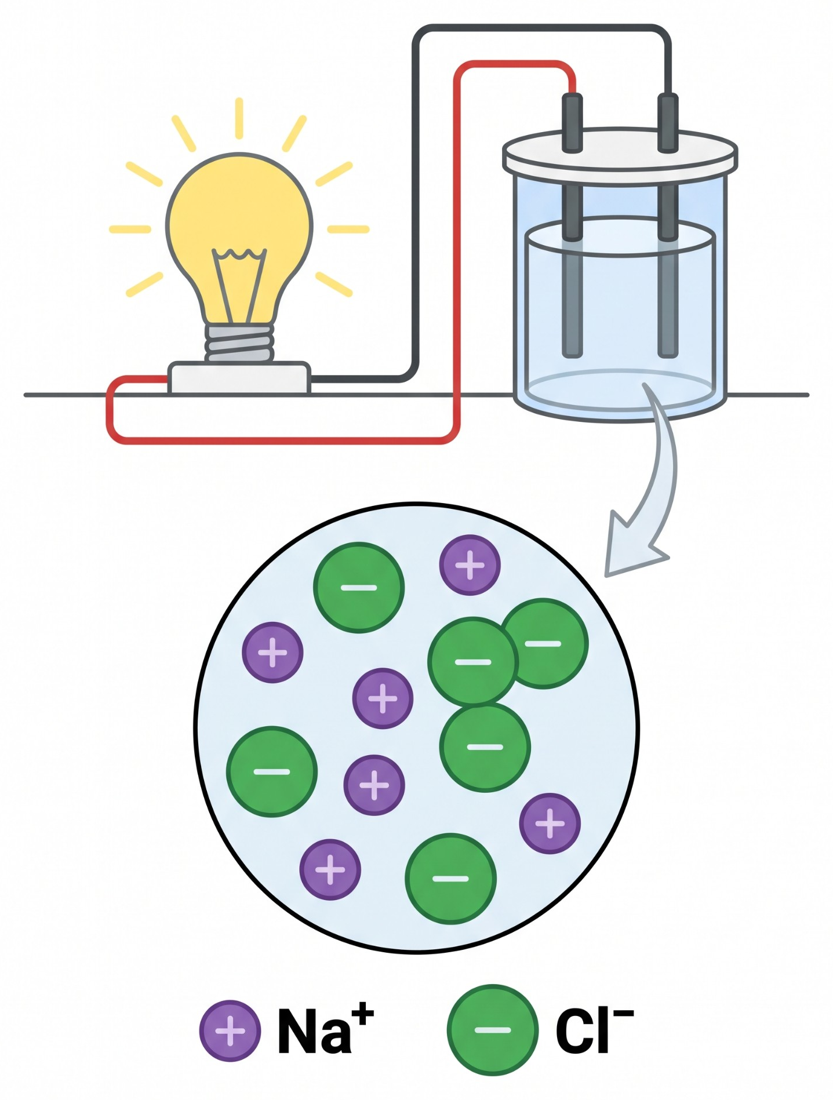
\includegraphics[width=0.86\linewidth]{rasmlar/darslik/d_elektr_asbob.png}\end{center}
\noindent A)~\textsl{eritmada erkin harakatlanuvchi ionlar hosil bo`ladi}\par
\noindent B)~\textsl{tuz suvda molekulalarga parchalanadi}\par
\noindent C)~\textsl{eritmada erkin elektronlar bor}\par
\noindent D)~\textsl{suv metall o`tkazgich   ---}\par
\qsep
\end{multicols}
\medskip
\noindent\setlength{\fboxsep}{0pt}\fbox{\begin{tabular}{p{0.74\linewidth}|p{0.2\linewidth}}
\parbox[t]{0.72\linewidth}{\vspace{3pt}\textbf{Topshiriqlar (33--35) va javob variant (A--F)larini o`zaro to`g`ri moslashtiring.} CaCO\textsubscript{3} va Na\textsubscript{2}CO\textsubscript{3} dan iborat 30,6 g aralashma mo`l xlorid kislota bilan reaksiyaga kirishdi. Ajralgan gaz 0,45 mol NaOH tutgan eritmadan o`tkazildi.
\vspace{3pt}} & \parbox[t]{0.19\linewidth}{\vspace{3pt}A~\textsl{13,44}\\[3pt]
B~\textsl{6,72}\\[3pt]
C~\textsl{10,08}\\[3pt]
D~\textsl{0,6}\\[3pt]
E~\textsl{5,38}\\[3pt]
F~\textsl{0,3}}\\ \hline
\parbox[t]{0.72\linewidth}{\vspace{2pt}\textbf{33. Ajralgan gazning hajmini (l, n.sh.) aniqlang.}\vspace{2pt}} & \\ \hline
\parbox[t]{0.72\linewidth}{\vspace{2pt}\textbf{34. Aralashmani to`liq eritish uchun sarflangan HCl miqdorini (mol) aniqlang.}\vspace{2pt}} & \\ \hline
\parbox[t]{0.72\linewidth}{\vspace{2pt}\textbf{35. Gaz NaOH eritmasidan o`tkazilganda hosil bo`lgan tuz (NaHCO\textsubscript{3}) massasini (g) aniqlang (reaksiya unumi 80\%).}\vspace{2pt}} & 
\end{tabular}}
\par\bigskip
\noindent\qn{36.} KMnO\textsubscript{4} + KI + H\textsubscript{2}SO\textsubscript{4} $\to$ MnSO\textsubscript{4} + I\textsubscript{2} + K\textsubscript{2}SO\textsubscript{4} + H\textsubscript{2}O reaksiya tenglamasini tenglang. Oksidlovchi va qaytaruvchi oldidagi koeffitsiyentlar \textbf{yig`indisini aniqlang.}
\javob\qsep
\noindent\qn{37.} H\textsubscript{2}SO\textsubscript{4} ning 0,025 mol/l li eritmasidan 0,4 l va Ba(OH)\textsubscript{2} ning 0,025 mol/l li eritmasidan 0,6 l aralashtirildi (umumiy hajm 1 l, ikkala modda to`liq dissotsilanadi, BaSO\textsubscript{4} cho`kmasi e'tiborga olinmasin). Hosil bo`lgan eritmaning pH \textbf{ini aniqlang.}
\javob\qsep
\noindent\qn{38.} NaBr va NaI dan iborat 28,1 g aralashma eritilib, mo`l xlor o`tkazildi, eritma bug`latilib quruq qoldiq 14,62 g chiqdi. Aralashmadagi NaI ning \textbf{massasini (g) toping.}
\javob\qsep
\noindent\qn{39.} Etilen va asetilendan iborat 4,48 l (n.sh.) aralashma bromli suvdan o`tkazilganda 40 g brom yutildi. Aralashmadagi asetilenning \textbf{hajmini (l, n.sh.) toping.}
\javob\qsep
\noindent\qn{40.} Alkanning vodorodga nisbatan zichligi 36, uglerodning massa ulushi 83,33\%. Shu alkan molekulasidagi $\sigma$-bog`lar umumiy \textbf{sonini toping.}
\javob\qsep
\par\bigskip\begin{center}\textbf{\fontsize{13}{15}\selectfont YOZMA ISH}\end{center}
\noindent\qn{41.} \textbf{Topshiriqni bajarish jarayonida barcha reaksiya tenglamalarini yozing. Miqdoriy va arifmetik hisoblashlarni (unga asos bo`lgan usul yoki formulani ko`rsatgan holda) uzviy ketma-ketlikda bajaring.}\par\smallskip
Tabiiy mis ikki izotopdan iborat: \textsuperscript{63}Cu (70\%) va \textsuperscript{65}Cu (30\%). 32 g shu element namunasi olingan (\textit{Z} = 29, N\textsubscript{A} = 6,02$\cdot$10\textsuperscript{23}).\par
\noindent 1)\ Elementning o`rtacha nisbiy atom massasini hisoblang.\par
\noindent 2)\ Namunadagi atomlarning umumiy miqdorini (mol) toping. Namunadagi protonlar sonini (mol) ham toping.\par
\noindent 3)\ Og`irroq izotop (\textsuperscript{65}Cu) atomlarining miqdorini (mol) hisoblang.\par
\noindent 4)\ Namunadagi neytronlarning umumiy miqdorini (mol) toping. Bitta atom massasini (g) ham hisoblang.\par
\noindent 5)\ Namunadagi atomlar sonini (10\textsuperscript{23} birligida) aniqlang. Namunadagi protonlar sonining neytronlar soniga nisbatini ham toping.\par
\diqqat{Mazkur topshiriq kengaytirilgan javobni talab etib, uning yechilish usuli va shu usul asosidagi barcha hisoblash amallari javoblar varaqasida aks etishi lozim.}\qsep
\noindent\qn{42.} Quyidagi o`zgarishlar zanjirida \textit{X}, \textit{Y}, \textit{Z} noma'lum organik moddalar:\par
\[\setlength{\fboxsep}{0pt}\text{C\textsubscript{2}H\textsubscript{5}Cl}\xrightarrow{\text{KOH (suvli)}}\text{\textit{X}}\xrightarrow{\text{H\textsubscript{2}SO\textsubscript{4} (kons.), 170 \textdegree{}C}}\text{\textit{Y}}\xrightarrow{\text{Br\textsubscript{2}}}\text{\textit{Z}}\xrightarrow{\text{KOH (spirtli)}}\text{C\textsubscript{2}H\textsubscript{2}}\]
\noindent 1)\ C\textsubscript{2}H\textsubscript{5}Cl $\to$ \textit{X} : reaksiya tenglamasini yozing; hosil bo`lgan moddani nomlang.\par
\noindent 2)\ \textit{X} $\to$ \textit{Y} : reaksiya tenglamasini yozing; hosil bo`lgan moddani nomlang.\par
\noindent 3)\ \textit{Y} $\to$ \textit{Z} : reaksiya tenglamasini yozing; hosil bo`lgan moddani nomlang.\par
\noindent 4)\ \textit{Z} $\to$ C\textsubscript{2}H\textsubscript{2} : reaksiya tenglamasini yozing; hosil bo`lgan moddani nomlang.\par
\diqqat{Mazkur topshiriq kengaytirilgan javobni talab etib, uning yechilish usuli va shu usul asosidagi barcha hisoblash amallari javoblar varaqasida aks etishi lozim.}\qsep
\noindent\qn{43.} \textbf{Topshiriqni bajarish jarayonida barcha reaksiya tenglamalarini yozing. Miqdoriy va arifmetik hisoblashlarni (unga asos bo`lgan usul yoki formulani ko`rsatgan holda) uzviy ketma-ketlikda bajaring.}\par\smallskip
CaCO\textsubscript{3} va MgCO\textsubscript{3} dan iborat 28,4 g aralashma doimiy massagacha qizdirildi. Ajralgan gaz mo`l Ca(OH)\textsubscript{2} eritmasidan o`tkazildi.\par
\noindent 1)\ Aralashmadagi har bir tuzning massasini (g) va massa ulushini (\%) aniqlang (reaksiya tenglamalarini yozing).\par
\noindent 2)\ Ajralgan gaz hajmini (l, n.sh.) va qattiq qoldiq massasini (g) toping. Qoldiqdagi CaO ning massa ulushini (\%) ham hisoblang.\par
\noindent 3)\ Gaz Ca(OH)\textsubscript{2} eritmasidan o`tkazilganda hosil bo`lgan cho`kma massasini (g) hisoblang.\par
\noindent 4)\ Qattiq qoldiqni to`liq eritish uchun 10\% li HCl eritmasidan necha gramm kerak?\par
\noindent 5)\ Qoldiq oksidlar suvga solinganda hosil bo`ladigan Ca(OH)\textsubscript{2} massasini (g) toping (CaO + H\textsubscript{2}O $\to$ Ca(OH)\textsubscript{2}).\par
\diqqat{Mazkur topshiriq kengaytirilgan javobni talab etib, uning yechilish usuli va shu usul asosidagi barcha hisoblash amallari javoblar varaqasida aks etishi lozim.}\qsep
\newpage
\noindent\textbf{\fontsize{13}{15}\selectfont 5-variant}\hfill \textbf{Javoblar kaliti}\par\smallskip\hrule\smallskip
\textit{Faqat o`qituvchi uchun.}\par\medskip
\noindent\textbf{1--32-savollar}\par\smallskip
\noindent\begin{tabular}{|c|c|c|c|c|c|c|c|c|c|c|c|c|c|c|c|}\hline
\textbf{1} & \textbf{2} & \textbf{3} & \textbf{4} & \textbf{5} & \textbf{6} & \textbf{7} & \textbf{8} & \textbf{9} & \textbf{10} & \textbf{11} & \textbf{12} & \textbf{13} & \textbf{14} & \textbf{15} & \textbf{16}\\\hline
\textsl{B} & \textsl{D} & \textsl{C} & \textsl{C} & \textsl{D} & \textsl{D} & \textsl{B} & \textsl{C} & \textsl{A} & \textsl{D} & \textsl{B} & \textsl{D} & \textsl{D} & \textsl{B} & \textsl{A} & \textsl{B}\\\hline
\textbf{17} & \textbf{18} & \textbf{19} & \textbf{20} & \textbf{21} & \textbf{22} & \textbf{23} & \textbf{24} & \textbf{25} & \textbf{26} & \textbf{27} & \textbf{28} & \textbf{29} & \textbf{30} & \textbf{31} & \textbf{32}\\\hline
\textsl{D} & \textsl{B} & \textsl{C} & \textsl{C} & \textsl{C} & \textsl{D} & \textsl{B} & \textsl{A} & \textsl{A} & \textsl{A} & \textsl{C} & \textsl{B} & \textsl{C} & \textsl{A} & \textsl{A} & \textsl{A}\\\hline
\end{tabular}\par\medskip
\noindent\textbf{33--35-savollar}\par\smallskip
\noindent\begin{tabular}{|c|c|c|}\hline \textbf{No} & \textbf{Javob} & \textbf{Qiymat}\\\hline
33 & \textsl{B} & 6,72\\\hline
34 & \textsl{D} & 0,6\\\hline
35 & \textsl{C} & 10,08\\\hline
\end{tabular}\par\medskip
\noindent\textbf{36--40-savollar}\par\smallskip
\noindent\begin{tabular}{|c|c|}\hline \textbf{No} & \textbf{To`g`ri javob}\\\hline
36 & 12\\\hline
37 & 12\\\hline
38 & 7,5\\\hline
39 & 1,12\\\hline
40 & 16\\\hline
\end{tabular}\par\medskip
\noindent\textbf{41--43-topshiriqlar: javoblar}\par\smallskip
\noindent\textbf{41-topshiriq.}\par
\noindent 1) 63,6\par
\noindent 2) 0,503 mol; 14,591 mol\par
\noindent 3) 0,151 mol\par
\noindent 4) 17,409 mol; 10,56$\cdot$10\textsuperscript{$-$23} g\par
\noindent 5) 3,03$\cdot$10\textsuperscript{23}; 0,838\par
\noindent\textbf{42-topshiriq.}\par
\noindent 1) C\textsubscript{2}H\textsubscript{5}Cl + KOH (suvli) $\to$ C\textsubscript{2}H\textsubscript{5}OH (etanol)\par
\noindent 2) C\textsubscript{2}H\textsubscript{5}OH + H\textsubscript{2}SO\textsubscript{4} (kons.), 170 \textdegree{}C $\to$ C\textsubscript{2}H\textsubscript{4} (etilen)\par
\noindent 3) C\textsubscript{2}H\textsubscript{4} + Br\textsubscript{2} $\to$ C\textsubscript{2}H\textsubscript{4}Br\textsubscript{2} (1,2-dibrometan)\par
\noindent 4) C\textsubscript{2}H\textsubscript{4}Br\textsubscript{2} + KOH (spirtli) $\to$ C\textsubscript{2}H\textsubscript{2} (asetilen)\par
\noindent\textbf{43-topshiriq.}\par
\noindent 1) x$\cdot$100 + y$\cdot$84 = 28,4; x + y = 0,3 $\to$ CaCO\textsubscript{3} 20 g (70,4\%), MgCO\textsubscript{3} 8,4 g (29,6\%)\par
\noindent 2) 6,72 l; 15,2 g; 73,7\%\par
\noindent 3) 30 g\par
\noindent 4) 219 g\par
\noindent 5) 14,8 g\par
\par\bigskip\noindent\textbf{Mavzular taqsimoti}\par\smallskip
{\small\noindent\begin{longtable}{|c|p{7.2cm}|p{5.4cm}|c|}\hline \textbf{No} & \textbf{Mavzu} & \textbf{Tekshiriladigan ko`nikma} & \textbf{Ball}\\\hline
1 & 9-sinf (gidroliz); Tirkashev IV bob & Bilim va tushunish & 1\\\hline
2 & Tirkashev VI bob (muvozanat, jadval) & Jadval tahlili & 1\\\hline
3 & Tirkashev VI bob (muvozanat, jadval) & Jadval tahlili & 1\\\hline
4 & 10-sinf \S{}17 (gibridlanish); Abdusamatov & Bilim va tushunish & 1\\\hline
5 & 7-sinf (Avogadro) & Hisoblash va masala yechish & 1\\\hline
6 & Tirkashev \textit{V} bob; 11-sinf 7-bob (OQR tenglash) & Hisoblash va masala yechish & 1\\\hline
7 & 11-sinf 8-bob; Tirkashev \textit{V} bob (elektroliz) & Bilim va tushunish & 1\\\hline
8 & Tirkashev VI bob (aktivlanish energiyasi, grafik) & Grafik tahlili & 1\\\hline
9 & 7-sinf (valentlik) & Bilim va tushunish & 1\\\hline
10 & Tirkashev I bob; 8-sinf (elektron konfiguratsiya) & Bilim va tushunish & 1\\\hline
11 & Tirkashev \textit{V} bob; Tashev (HNO\textsubscript{3}, H\textsubscript{2}SO\textsubscript{4}) & Hisoblash va masala yechish & 1\\\hline
12 & 10-sinf \S{}17 & Bilim va tushunish & 1\\\hline
13 & Tirkashev VI bob (kimyoviy muvozanat) & Hisoblash va masala yechish & 1\\\hline
14 & Tashev (nodir gazlar); 8-sinf & Bilim va tushunish & 1\\\hline
15 & Tashev (nitratlar termik parchalanishi) & Hisoblash va masala yechish & 1\\\hline
16 & 9-sinf; Tashev (anorganik birikmalar xossalari) & Bilim va tushunish & 1\\\hline
17 & Tashev (HNO\textsubscript{3} olinishi) & Hisoblash va masala yechish & 1\\\hline
18 & 9-sinf (uglerod (IV) oksid) & Hisoblash va masala yechish & 1\\\hline
19 & Tashev (HCl olinishi) & Hisoblash va masala yechish & 1\\\hline
20 & 10-sinf (arenlar) & Rasm bo`yicha tahlil & 1\\\hline
21 & 10-sinf (mavzuga oid paragraflar); Abdusamatov & Bilim va tushunish & 1\\\hline
22 & 10-sinf (mavzuga oid paragraflar); Abdusamatov & Bilim va tushunish & 1\\\hline
23 & 10-sinf (spirt, hisob) & Hisoblash va masala yechish & 1\\\hline
24 & 10-sinf \S{}24; \S{}26; \S{}30 (kumush ko`zgu) & Hisoblash va masala yechish & 1\\\hline
25 & 10-sinf (mavzuga oid paragraflar); Abdusamatov & Bilim va tushunish & 1\\\hline
26 & 10-sinf (mavzuga oid paragraflar); Abdusamatov & Bilim va tushunish & 1\\\hline
27 & 10-sinf (ugl, hisob) & Hisoblash va masala yechish & 1\\\hline
28 & 10-sinf (mavzuga oid paragraflar); Abdusamatov & Bilim va tushunish & 1\\\hline
29 & 10-sinf (mavzuga oid paragraflar); Abdusamatov & Bilim va tushunish & 1\\\hline
30 & Tirkashev III bob; 7-sinf (eritma tayyorlash) & Hisoblash va masala yechish & 1\\\hline
31 & 7-sinf (aralashmalarni ajratish usullari) & Bilim va tushunish & 1\\\hline
32 & 9-sinf (elektrolitlar, 1-rasm) & Rasm bo`yicha tahlil & 1\\\hline
33--35 & Aralash masala (moslashtirish) & Ko`p bosqichli hisob & 3\\\hline
36--40 & Qisqa javobli masalalar & Hisoblash & 5\\\hline
41--43 & Yozma ish & Usul va hisob (M, A) & 75\\\hline
\end{longtable}}
\end{document}
